\documentclass[a4paper]{article}

\input ../header
\usepackage{minted}
\usepackage[np]{numprint}
\usepackage{lscape}
\usepackage{afterpage}
\usepackage{hyperref}

\setlength{\multicolsep}{2pt}

% Commandes pour cacher/révéler du texte facilement à l'aide d'un booléen
\usepackage{xstring}
\usepackage{ifthen}

\newboolean{reveal}
\setboolean{reveal}{false}

\newlength{\stextwidth} % une nouvelle longueur

\newcommand\x{6}

\newcommand{\guess}[1]{\ifthenelse{\boolean{reveal}}{{\color{red}#1}}{\settowidth{\stextwidth}{#1}\makebox[\stextwidth]{\dotfill}}}

\newcommand{\guessmath}[1]{\ifthenelse{\boolean{reveal}}{\textcolor{red}{#1}}{\settowidth{\stextwidth}{$#1$}\makebox[1.9\stextwidth]{\dotfill}}}

\newcommand{\guessmathbin}[1]{\ifthenelse{\boolean{reveal}}{\mathbin{\color{red}#1}}{\settowidth{\stextwidth}{$#1$}\makebox[2\stextwidth]{\dotfill}}}

\begin{document}

\title{Le Web -- Activité 1}

\pagestyle{empty}

\date{}
\author{}

\maketitle{}

\thispagestyle{empty}
\noindent\textbf{Activité 1}\hfill{}\textbf{Enjeux éthiques et sociétaux du Web}
\smallskip
\hrule
\medskip

L'usage du Web tend à s'imposer dans notre quotidien. Cela n'est pas sans conséquences sur chacune de nos personnalités et sur nos modes de sociabilité.

\begin{center}
  Quels sont les impacts de l'évolution du Web sur l'individu et la société ?
\end{center}

\medskip

\textbf{Document 1 -- Accès généralisé à la publication et à la diffusion} 

\begin{multicols}{2}
  \begin{center}
    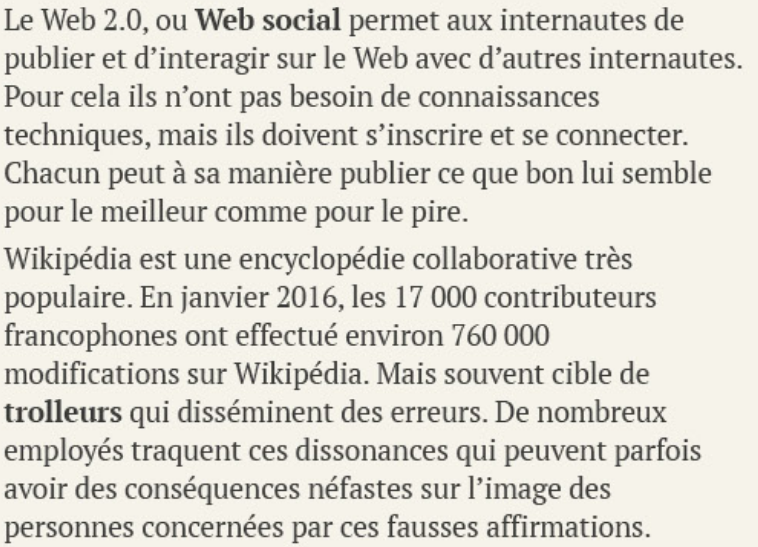
\includegraphics[width=9cm]{web_2.0.png}
  \end{center}\columnbreak

  \vspace*{-3mm}

  \begin{enumerate}
    \item Qu'est-ce qu'un troll/trolleur ?\rep{4}
    \item Citer un avantage de l'édition collaborative.\rep{4}
    \item En citer un inconvénient.\rep{4}
  \end{enumerate}
\end{multicols}

\bigskip

\textbf{Document 2 -- Législation encadrant les publications sur le Web} 

\smallskip

\begin{multicols}{2}
  \begin{enumerate}[resume]
    \item Que dit l'article 1 de la loi du 29 juillet 1881 sur la liberté de la presse ?\rep{5}
    \item À quel article de la Déclaration des droits de l'homme et du citoyen cet article fait-il écho ?\rep{5}
  \end{enumerate}

  \begin{center}
    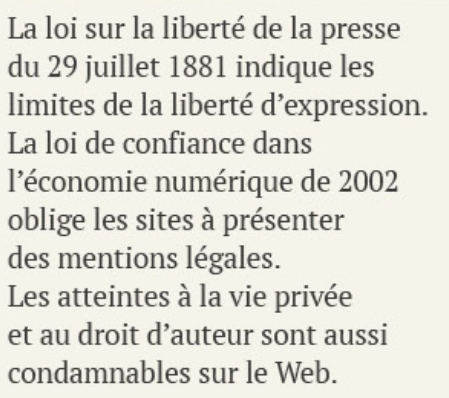
\includegraphics[width=7cm]{legislation_publications_web.png}
  \end{center}
\end{multicols}

\begin{enumerate}
  \setcounter{enumi}{5}
\item Que dit la loi pour la confiance dans l'économie numérique en matière de publicité électronique (par email par exemple) ?\rep{6}
\end{enumerate}

\pagebreak

\textbf{Document 3 -- Personnalisation de l'expérience utilisateur} 

\medskip

\begin{multicols}{2}
  \begin{center}
    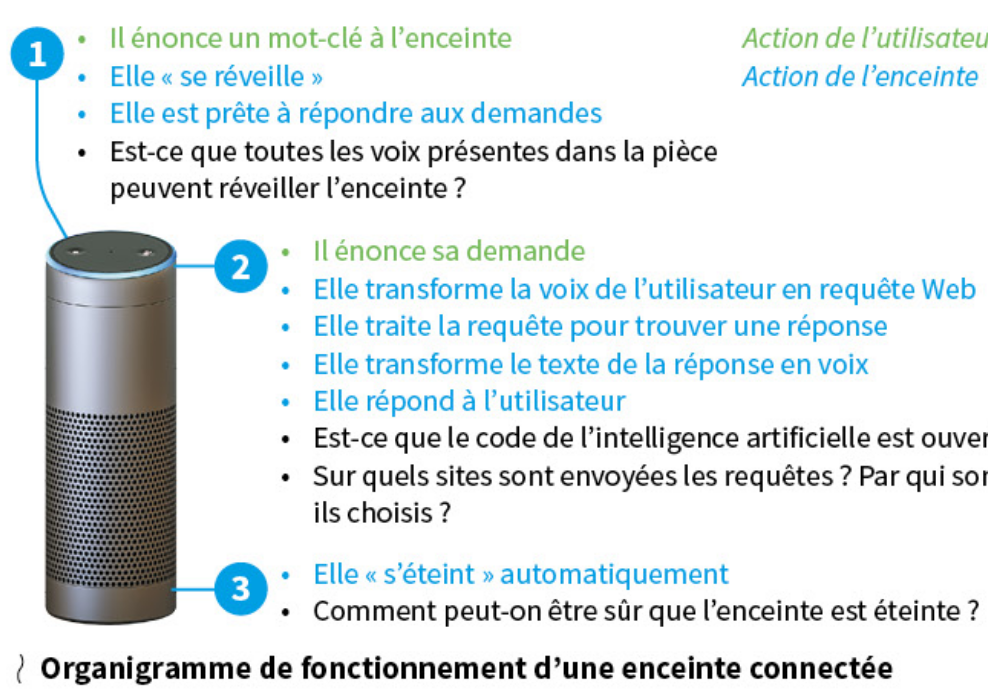
\includegraphics[width=9cm]{enceinte_connectee.png} 
  \end{center}\columnbreak
  \begin{enumerate}[resume]
    \item Donner deux exemples d'enceintes connectées.\rep{4}
    \item Donner un avantage de posséder une enceinte connectée.\rep{4}
    \item Donner un inconvénient d'en posséder une en citant un fait divers récent.\rep{4}
  \end{enumerate}
\end{multicols}

\bigskip

\textbf{Document 4 -- Retenir l'attention des internautes} 

\begin{center}
  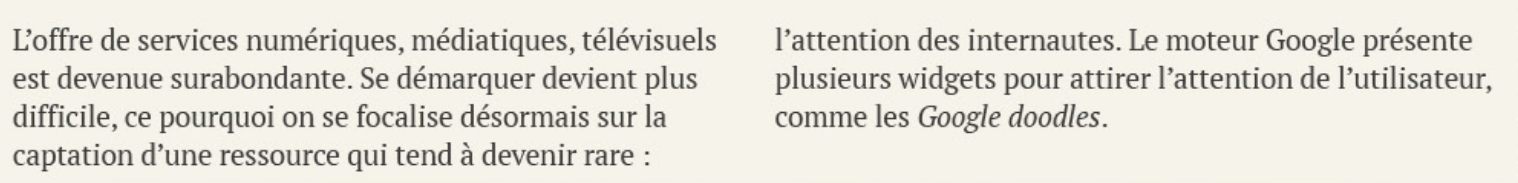
\includegraphics[width=16cm]{attention_internautes.png}
\end{center}

\begin{enumerate}[resume]
  \setcounter{enumi}{9}
  \item Qu'est-ce qu'un \textit{Google Doodle} ?\rep{3}
  \item Chercher la définition d'\textit{infinite scroll}.\rep{3}
  \item Q'est-ce qu'une \textit{notification push} ?\rep{3}
\end{enumerate}

\bigskip

\textbf{Document 5 -- En 2019, les 30 ans de l'invention du Web} 

\begin{center}
  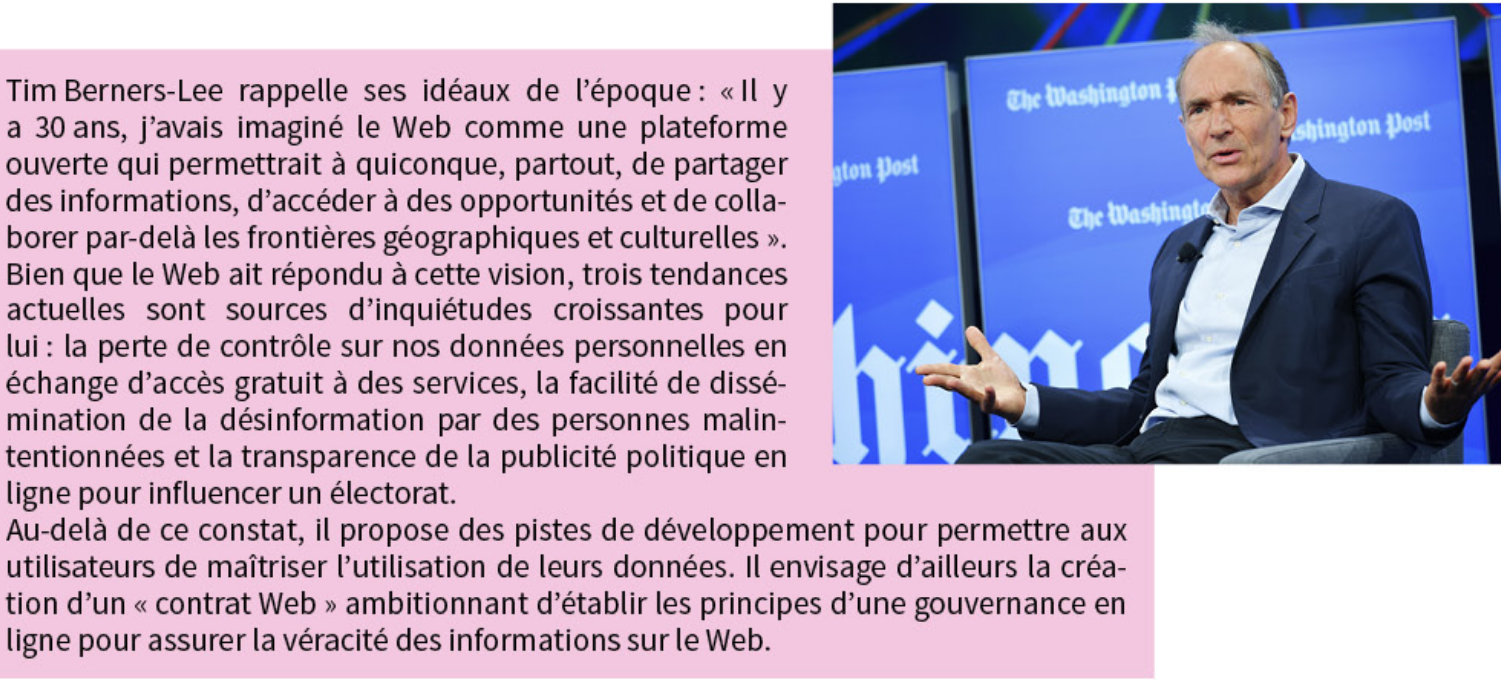
\includegraphics[width=16cm]{tim_berners-lee_entrevue_washington_post.png}
\end{center}

\begin{enumerate}
  \setcounter{enumi}{12}
  \item Le document ci-dessus est tiré d'une entrevue accordée par Tim Berners-Lee au Washington Post. Quelles inquiétudes Tim Berners-Lee partage-t-il ?\rep{6}
  \item On retrouve parfois ce message sur le mur de certains utilisateurs du réseau social Facebook :

    \begin{center}
      \textit{N'oubliez pas la date limite demain !!! Tout ce que vous avez publié devient public à partir de demain. Même les messages qui ont été supprimés ou les photos qui n'ont pas été autorisées. Ça ne coûte rien pour une simple copie et coller, mieux vaut que désolé. Channel 13 news a parlé du changement dans la politique de protection de la vie privée de Facebook. Je ne donne à Facebook ni à aucune entité associée à Facebook l'autorisation d'utiliser mes photos, informations, messages ou publications, à la fois passé et futur. Avec cette déclaration, je fais remarquer à Facebook qu'il est strictement interdit de divulguer, de copier, de distribuer ou de prendre toute autre action contre moi en fonction de ce profil et / ou de son contenu. Le contenu de ce profil est des informations privées et confidentielles. La violation de la vie privée peut être punie par la loi (UCC 1-308-1 1 308-103 et le statut de Rome).}
    \end{center}

    \begin{enumerate}[resume]
      \item Pourquoi ces utilisateurs publient-ils ce message ?\rep{4}
      \item Que penser de son utilité ?\rep{4}
    \end{enumerate}
  \item Résumer en quelques phrases le scandale Facebook-Cambridge Analytica.\rep{4}
\end{enumerate}
\end{document}
